\documentclass[fontsize=12pt,paper=a4,twoside]{scrartcl}

\newcommand{\grad}{\ensuremath{^{\circ}} }
\renewcommand{\strut}{\vrule width 0pt height5mm depth2mm}

\usepackage[utf8]{inputenc}
\usepackage[final]{pdfpages}
% obere Seitenränder gestalten können
\usepackage{fancyhdr}
\usepackage{moreverb}
% Graphiken als jpg, png etc. einbinden können
\usepackage{graphicx}
\usepackage{stmaryrd}
% Floats Objekte mit [H] festsetzen
\usepackage{float}
% setzt URLs schön mit \url{http://bla.laber.com/~mypage}
\usepackage{url}
% Externe PDF's einbinden können
\usepackage{pdflscape}
% Verweise innerhalb des Dokuments schick mit " ... auf Seite ... "
% automatisch versehen. Dazu \vref{labelname} benutzen
\usepackage[ngerman]{varioref}
\usepackage[ngerman]{babel}
\usepackage{ngerman}
% Bibliographie
\usepackage{bibgerm}
% Tabellen
\usepackage{tabularx}
\usepackage{supertabular}
\usepackage[colorlinks=true, pdfstartview=FitV, linkcolor=blue,
            citecolor=blue, urlcolor=blue, hyperfigures=true,
            pdftex=true]{hyperref}
\usepackage{bookmark}

\newboolean{langversion} %Deklaration
\setboolean{langversion}{true} %Zuweisung ist 'false' für Blockkurs
\newcommand{\highlight}[1]{\textcolor{blue}{\textbf{#1}}}
\newcommand{\nurlangversion}[0]{%
\ifthenelse{\boolean{langversion}}{\highlight{Muss in SWP-2 ausgefüllt werden}}{\highlight{Entfällt in SWP-1}}}

\newcommand{\swp}[0]{\ifthenelse{\boolean{langversion}}%
{Software--Projekt 2}{Software--Projekt 1}}
\newcommand{\jahr}[0]{2013}
\newcommand{\semester}[0]{\ifthenelse{\boolean{langversion}}{WiSe}{SoSe} \jahr}

% Damit Latex nicht zu lange Zeilen produziert:
\sloppy
%Uneinheitlicher unterer Seitenrand:
%\raggedbottom

% Kein Erstzeileneinzug beim Absatzanfang
% Sieht aber nur gut aus, wenn man zwischen Absätzen viel Platz einbaut
\setlength{\parindent}{0ex}

% Abstand zwischen zwei Absätzen
\setlength{\parskip}{1ex}

% Seitenränder für Korrekturen verändern
\addtolength{\evensidemargin}{-1cm}
\addtolength{\oddsidemargin}{1cm}

\bibliographystyle{gerapali}

% Lustige Header auf den Seiten
  \pagestyle{fancy}
  \setlength{\headheight}{70.55003pt}
  \fancyhead{}
  \fancyhead[LO,RE]{\swp\\ \semester{}
  \\Anforderungsspezifikation}
  \fancyhead[LE,RO]{Seite \thepage\\\slshape \leftmark\\\slshape \rightmark}

%
% Und jetzt geht das Dokument los....
%

\begin{document}

% Lustige Header nur auf dieser Seite
  \thispagestyle{fancy}
  \fancyhead[LO,RE]{ }
  \fancyhead[LE,RO]{Universität Bremen\\FB 3 -- Informatik\\
  Prof. Dr. Rainer Koschke \\TutorIn: Sabrina Wilske}
  \fancyfoot[C]{}

% Start Titelseite
  \vspace{3cm}

  \begin{minipage}[H]{\textwidth}
  \begin{center}
  \bf
  \Large
  \swp{} \jahr\\
  \smallskip
  \small
  VAK 03-BA-901.02\\
  \vspace{3cm}
  \end{center}
  \end{minipage}
  \begin{minipage}[H]{\textwidth}
  \begin{center}
  \vspace{1cm}
  \bf
  {\Large Anforderungsspezifikation}\\
  \vspace{3ex}
  \small IT\_R3V0LUT10N\\
  \vfill
  \end{center}
  \end{minipage}
  \vfill
  \begin{minipage}[H]{\textwidth}
  \begin{center}
  \sf
  \begin{tabular}{lrr}
  Sebastian Bredehöft & sbrede@tzi.de & 2751589\\
  Patrick Damrow & damsen@tzi.de & 2056170\\
  Tobias Dellert & tode@tzi.de & 2936941\\
  Tim Ellhoff & tellhoff@tzi.de & 2520913\\
  Daniel Pupat & dpupat@tzi.de & 2703053\\
  \end{tabular}
  \\ ~
  \vspace{2cm}
  \\
  \it Abgabe: 17. November 2013 --- Version 1.1\\ ~
  \end{center}
  \end{minipage}

% Ende Titelseite

% Start Leerseite

\newpage

  \thispagestyle{fancy}
  \fancyhead{}
  \fancyhead[LO,RE]{\swp{}\\ \semester{} \jahr{}
  \\Anforderungsspezifikation}
  \fancyhead[LE,RO]{Seite \thepage\\\slshape \leftmark\\~}
  \fancyfoot{}
  \renewcommand{\headrulewidth}{0.4pt}
  \tableofcontents

\newpage

  \fancyhead[LE,RO]{Seite \thepage\\\slshape \leftmark\\\slshape \rightmark}


%%%%%%%%%%%%%%%%%%%%%%%%%%%%%%%%%%%%%%%%%%%%%%%%%%%%%%%%%%%%%%%%%%%%%%%%
\section*{Version und Änderungsgeschichte}

{\em Die aktuelle Versionsnummer des Dokumentes sollte eindeutig und gut zu
identifizieren sein, hier und optimalerweise auf dem Titelblatt.}

\begin{tabular}{ccl}
Version & Datum & Änderungen \\
\hline
1.0 & TT.MM.JJJJ & Projektplan als \LaTeX Vorlage kopiert. \\
1.1 & 31.10.2013 & Charakteristika der Benutzer \\
1.2 & 01.11.2013 & System- und Hardwareschnittstellen \\
\end{tabular}


%%%%%%%%%%%%%%%%%%%%%%%%%%%%%%%%%%%%%%%%%%%%%%%%%%%%%%%%%%%%%%%%%%%%%%%%
\section{Einleitung}
\nurlangversion

{\em Dieses Dokument dient als Vorlage für Eure
  Anforderungsspezifikation. Die Gliederung dieses
  Dokuments ist an die Struktur des IEEE-Standards 830.1998 angelehnt,
  weicht jedoch an einigen Stellen davon ab. Die Abweichungen sind
  im weiteren Verlauf dieses Dokuments dokumentiert. Weitere detaillierte
  Hinweise finden sich im IEEE-Standard 830.1998, der in Stud.IP      
  beziehungsweise über die Uni-Bibliothek in digitaler Form verfügbar ist
  \footnote{Bei \url{http://ieeexplore.ieee.org} im Suchfeld 'IEEE std    
   830-1998' eingeben. Funktioniert nur innerhalb des Uni-Netzes.}.}

\subsection{Zweck}
\nurlangversion

  {\em Was ist der Zweck dieser Anforderungsspezifikation? Wer sind
  die LeserInnen?}

\subsection{Rahmen}
\nurlangversion

  {\em Dieser Abschnitt soll einen groben Überblick über die zu
  erstellende Software geben: Welche Produkte sind zu erstellen (mit
  Namen)? Was tut die Software? Auch: Was tut sie nicht? Wozu soll die
  Software verwendet werden?  (Ziele etc.)}

\subsection{Definitionen, Akronyme und Abkürzungen}
\nurlangversion

  {\em Hier geht es vor allem um Begriffe aus der Anwendungsdomäne,
  d.h.\ aus der Welt des Kunden. Aber auch Begriffe, die dem Kunden
  evtl.\ fremd oder unklar sind, sollten erläutert werden.}


\subsection{Referenzen}
  {\em Neben sonstigen Quellen, die Ihr verwendet habt, können dies
  z.B.\ das Skript, dieses Beispieldokument, der zugrunde
  liegende IEEE-Standard und anderes sein}
  

\subsection{Übersicht über das Dokument}
\nurlangversion

  {\em Was enthält die Anforderungsspezifikation? Wie ist das Dokument
  organisiert?}


\section{Allgemeine Beschreibung}
\label{ch:AllgemeineBeschreibung}

\subsection{Ergebnisse der Ist-Analyse}
\nurlangversion

  {\em Hier sollten die Ergebnisse Eurer Ist-Analyse kurz
  zusammengefasst werden. Diese Beschreibung ist hilfreich, um die
  Motivation für die Anforderungen zu verstehen und um sie später
  nachzuvollziehen (z.B.\ dann wenn Anforderungen überarbeitet werden
  sollen, weil sich ihre Rahmenbedingungen geändert haben).
  
  Mögliche Inhalte: 
  \begin{itemize}
    \item Interview/Beobachtung des Kunden oder der Benutzer
    \item Analyse des bisherigen Systems und dessen Probleme 
    \item Analyse ähnlicher Systeme
    \item Auswertung der Benutzerbefragung
    \item Wie sollen die identifizierten Probleme vom neuen System adressiert werden?
  \end{itemize}
  
  N.B.: Dieser Abschnitt ist im IEEE-Standard nicht vorgesehen, aber dennoch
  sinnvoll.}

\subsubsection{Erstes Kundengespräch vom TT.MM.JJJJ}
\nurlangversion

\subsubsection{Interview mit einem Mitarbeiter der ...}
\nurlangversion

{\em Falls durchgeführt}

\subsection{Produktperspektive}
  
\subsubsection{Systemschnittstellen}

  {\em Schnittstellen zu anderen Systemen, z.B.\ Datenimport/-export,
  Konfigurationsdateien, anzubindende externe Dienste und deren Schnittstelle,
  Anbieten der eigenen Funktionalität als API o.ä.}
  
  
  \textbf{CSV-Im-/Export:}\\
  Es gibt eine Funktion, mithilfe dieser CSV-Dateien importiert werden können. Diese kann nur vom Administrator benutzt werden. Die Bücher werden anschließend in der Datenbank der Bibliothek vorhanden sein. \\
  Es ist auch möglich CSV Dateien zu exportieren, welche dann abgespeichert werden.

\subsubsection{Benutzerschnittstelle}
\nurlangversion

  {\em GUI-Design-Richtlinien und Interaktionsmechanismen (nicht
  Screenshots aller Dialoge --- die werden in Kapitel 3 gezeigt --- aber
  evtl.\ ein Screenshot, der einen groben Überblick und Eindruck des
  GUI-Designs gibt).}


\subsubsection{Hardwareschnittstellen}

  {\em Schnittstellen zu vorgegebenen Hardwarekomponenten (Name,
  Version).}
  
  \textbf{Computer:}\\
  Unser System soll auf einem Web-Browser laufen. Dabei sollte das System auf Windows laufen, welches die verwendete Plattform des Kunden ist. Dabei ist wchtig, das Windows 2000 bis Windows 8 unterstützt werden, da der Kunde Windows 2000 verwendet. Ebenfalls sollte das System Linux und MacOS unterstützen.\\
  \textbf{Smartphone:}\\
  Unser System unterstützt nur Geräte auf denen Android läuft. Dabei muss  die Version 2.3 oder höher vorliegen, da somit der größte Teil der Android Geräte verwendet werden kann.\\
 

\subsubsection{Softwareschnittstellen}
\nurlangversion

{\em Softwarebibliotheken und --rahmenwerke (Frameworks), die benutzt
  werden sollen, mit Versionsnummer, Hersteller, Quelle etc. Dazu
  gehört auf jeden Fall Java.}

  \begin{tabular}{|l|l|l|l|}\hline
    \textbf{Name} & \textbf{Version} & \textbf{Hersteller} & \textbf{Quelle} \\\hline
    Java Runtime & 6 Update 37 & Oracle & \url{http://java.com} \\\hline
    Hibernate & 4.3.0.Beta1 Release& JBoss Community &  
   \url{http://www.hibernate.org/}\\\hline
    \ldots & & & \\\hline
  \end{tabular}

\subsubsection{Kommunikationsschnittstellen}
\nurlangversion

{\em Anforderungen an und Bandbreite von Kommunikationsnetzwerken, öffentliche
  oder auch private IP-Adressen?}

\subsubsection{Speicherbeschränkung}
\nurlangversion

  {\em min./max.\ verfügbarer Hauptspeicher und Festplattenplatz, knappe Begründung wie Ihr zu
der hier angegebenen Einschätzung gekommen seid}

\subsubsection{Operationen (Betriebsmodi)}
\nurlangversion

  {\em Welche Betriebsmodi gibt es? Warum? Welche Benutzerklasse darf
  was in welchem Betriebsmodus (Rechte)? Was ist der Zusammenhang
  zwischen Betriebsmodus und Sicherung/Wiederherstellung von Daten?}

\subsubsection{Möglichkeiten der lokalen Anpassung}
\nurlangversion

  {\em Was kann bei Auslieferung des Systems alles konfiguriert
  werden? Z.B. Pfade, Datenbankname, Server-IP usw. Hier ist nicht
  Internationalisierung gemeint!}


\subsection{Anwendungsfälle}
  {\em Auflistung und kurze Beschreibung aller relevanten
  Anwendungsfälle. Dies soll einen Überblick über alle Anwendungsfälle
  geben, die in 3.2 detailliert beschrieben werden.}
  
\begin{itemize}
  \item \textbf{1. Programm starten}\\
  Website wird aufgerufen/ App wird gestartet. 
  \item \textbf{2. Benutzer anmelden}\\
  Ein Benutzer meldet sich an.
  \item \textbf{3. Benutzer abmelden}
  Ein Benutzer meldet sich ab.
  \item \textbf{4. Start anzeigen}
  \item \textbf{4.1 Leserprofil anzeigen}
  \item \textbf{4.1.1 Vormerkung bearbeiten}
  \item \textbf{5. Publikationen anzeigen}
  \item \textbf{6. Buch hinzufügen}
  \item \textbf{7. Buch ändern}
  \item \textbf{8. Buch löschen}
  \item \textbf{9. CVS-Import}
  \item \textbf{10. CVS-Export}
  \item \textbf{11. Buch suchen}
  \item \textbf{12. Einzelnes Buch anzeigen/ Detailansicht}
  \item \textbf{13. Buch bewerten}
  \item \textbf{14. Buch ausleihen}
  \item \textbf{14.1 Buchrückgabe}
  \item \textbf{15. Buch rezensieren}
  \item \textbf{16. Buch vormerken}
  \item \textbf{17. Rezension freischalten}
  \item \textbf{18. Leserliste anzeigen}
  \item \textbf{19. Leser hinzufügen}
  \item \textbf{20. Leser ändern}
  \item \textbf{21. Leser löschen}
  \item \textbf{22. CVS-Import}
  \item \textbf{23. CVS-Export}
  \item \textbf{24. Einzelnen Leser anzeigen/ Detailansicht}
  \item \textbf{24.1 Leser sperren}
  \item \textbf{25. Leser suchen}
  \item \textbf{26. Administration öffnen}
  \item \textbf{27. Bibliothekarliste anzeigen}
  \item \textbf{28. Bibliothekar hinzufügen}
  \item \textbf{29. Bibliothekar löschen}
  \item \textbf{30. Bibliothekar ändern}
  \item \textbf{31. Statistiken anzeigen}
  \item \textbf{32. Mahnungsliste anzeigen}
  \item \textbf{33. Mahnungsliste drucken}
  \item \textbf{34. Mahnungsdetails anzeigen}
  \item \textbf{35. Startseite bearbeiten}
  \item \textbf{36. Abgabedaten und Mahngebühren bearbeiten}
 \end{itemize}


\subsection{Charakteristika der Benutzer (Daniel)}
  {\em Beschreibt hier Eure typischen Benutzer. Benutzt dazu die in
  der Vorlesung vorgestellten Personas. Zur Erinnerung: Ihr beschreibt
  konkrete Personen, die Repräsentanten der verschiedenen
  Benutzertypen sind (mit Name, evtl. Wohnort, Tätigkeit, Alter, Bild,
  \ldots). Diese sollten eine gewisse Motivation haben, bestimmte
  Anwendungsfälle durchzuführen (und dort auch eingesetzt werden!).}


\begin{table}[htbp]
\caption{Benutzer}
\label{benutzer}
\begin{tabular}{|p{2,5cm}|p{2,8cm}|p{2,8cm}|p{2,8cm}|p{2,8cm}|}
\hline 
\textbf{Name(fiktiv)} & Bert Bib & Arnold Admin & Silke Schüler & Bart Besucher\\ \hline
\textbf{Bild(fiktiv)} & & & & \\ \hline
\textbf{Rolle} & Bibliothekar & Administrator & Leiherin & uregistrierter Leiher \\ \hline
\textbf{Beruf} & Bibliothekar & Bibliothekar & Schülerin & Anwalt\\ \hline
\textbf{Alter} & 39 & 56 & 16 & 34\\ \hline
\textbf{Ziel} & Bibliothek verwalten & System verwalten & Bücher ausleihen & Bücher ausleihen \\ \hline
\textbf{Verwendung der Software} & Bücher und Nutzer verwalten & System und Bibliothekare verwalten & Bücher suchen, ausleihen etc. & keine\\ \hline
\end{tabular}
\end{table}

\subsection{Einschränkungen}
\label{sec:Einschraenkungen}
  {\em Dinge, die die Entwurfsfreiheit einschränken, z.B.
  \begin{itemize}
   \item feste Vorgaben (z.B. Policies)
   \item gesetzliche Rahmenbedingungen
   \item Hardwarebeschränkungen
   \item festgelegte Schnittstellen zu anderen Anwendungen
   \item parallele Operationen (z.B. Multithreading)
   \item Prüfungs- und Steuerungsfunktionen
   \item Verlässlichkeitsanforderungen
   \item Kritikalität der Anwendung
   \item Sicherheit
  \end{itemize}
  }

\subsubsection{Rahmenbedingungen}
\nurlangversion

\subsubsection{Gesetzliche Rahmenbedingungen}
\nurlangversion
 
\subsubsection{Sicherheitskritische Aspekte}
\nurlangversion

\subsection{Annahmen und Abhängigkeiten}
\nurlangversion

  {\em Faktoren, deren Änderung zwangsläufig zu Änderungen an der
  Anforderungsspezifikation führen würde.}



\subsection{Ausblick}
\nurlangversion

  {\em Beschreibt hier knapp, welche Änderungen und Erweiterungen
  zukünftig (d.h.\ nach Auslieferung des Systems) zu erwarten sind.
  Diese Information ist wichtig für den Entwurf, um mögliche
  Änderungen frühzeitig im ersten Entwurf berücksichtigen zu können.
  Der Entwurf kann dann so gestaltet werden, dass die zukünftigen
  Anforderungen leicht realisierbar sind. Die zukünftigen
  Anforderungen sollten realistisch sein, ansonsten könnte ein unnötig
  allgemeiner und damit zu komplizierter Entwurf die Folge sein.  Auch
  dieser Abschnitt ist im IEEE-Standard nicht vorgesehen -- zumindest
  nicht explizit in Form eines eigenständigen Abschnitts. Dennoch
  handelt es sich um wertvolle Information, von der der Entwurf
  profitieren kann.}
  

\section{Detaillierte Beschreibung}
\label{ch:DetaillierteBeschreibung}
{\em Die externen Schnittstellen werden grob in Abschnitt 2
  beschrieben.  Wenn die grobe Beschreibung dort nicht genügt, kann
  sie hier detaillierter ausgeführt werden (wie vom IEEE-Standard
  vorgesehen).}

\subsection{Datenmodell}
  {\em Das Datenmodell im Kontext des Pflichtenhefts ist {\glqq}die
  Darstellung von Informationen und deren Beziehungen in einem
  fachlogischen Konzept{\grqq}. Es soll hier gezeigt werden, welche
  Einheiten für das existierende System relevant sind und welche
  Beziehungen zwischen diesen Einheiten gelten. Es handelt sich
  hierbei noch nicht um ein Datenbankschema oder eine Spezifikation
  von Klassen für die Implementierung (Entwurf), sondern um die
  Modellierung der realen Welt. Das Datenmodell ist leitend für den
  Entwurf (weil alles darin beschrieben sich auch in der Software 
  wiederfinden wird), aber nimmt den Entwurf nicht schon vorweg.
  
  Das Datenmodell soll als UML-Klassendiagramm angegeben werden.
  Wichtig ist hierbei die korrekte Verwendung der UML: Klassen,
  Attribute, Generalisierung, Assoziation, Aggregation, Komposition,
  Multiplizitäten. Außerdem sollte das Diagramm sinnvoll und gut
  lesbar sein. Dazu gehört weiterhin eine kurze Beschreibung des
  Modells mit ergänzenden Informationen, insbesondere wenn die
  Relationen durch ihren Namen nicht selbsterklärend sind. Gebt
  unbedingt ein Mengengerüst für die Daten an: Wie viele Instanzen der
  wichtigsten Klassen werden erwartet? Erwartet Ihr Änderungen im
  Datenvolumen in der Zukunft?}


\subsection{Anwendungsfälle}
\begin{figure}[htbp]
\caption{Startseite}
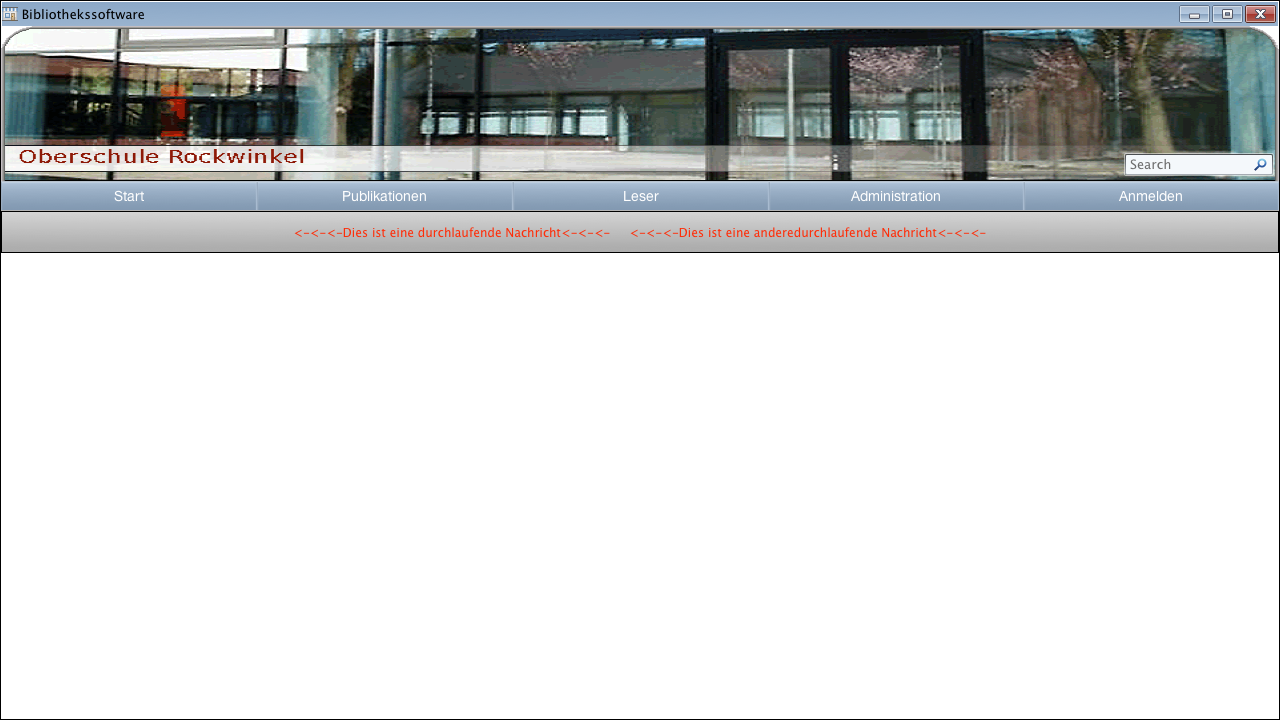
\includegraphics[width=1\textwidth]{WebApp-Screens/Startscreen-loggedOut.png}
  \label{startseite}
\end{figure}

\begin{table}[htbp]
\label{1}
\begin{tabular}{|l|p{10cm}|}
\hline 
\textbf{1} & \textbf{Programm starten} \\ \hline
\textbf{Akteure} & Bert Bib, Arnold Admin, Silke Schüler, Bart Besucher\\ \hline
\textbf{Ziel} & Der Akteur möchte das Programm starten  \\ \hline
\textbf{Vorbedingungen} & keine \\ \hline
\textbf{Regulärer Ablauf} & 
1. Der Akteur startet das Programm \\
&2. Das Programm startet und zeigt die Startseite \\ \hline
\textbf{Varianten} & keine \\ \hline
\textbf{Nachbedingungen} & Das Programm ist gestartet und der Benutzer kann dieses nun verwenden \\ \hline
\textbf{Fehler-/Ausnahmefälle} & keine \\ \hline
\end{tabular}
\end{table}

\begin{figure}[htbp]
\caption{Loginscreen}
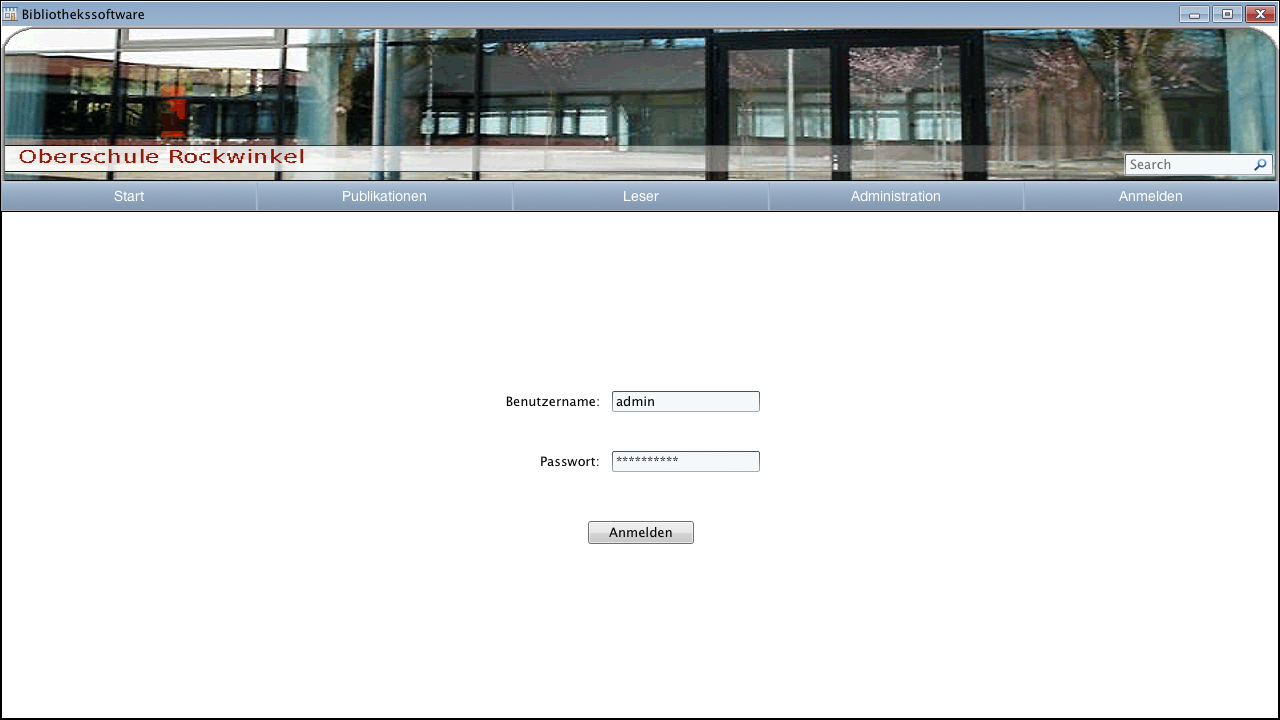
\includegraphics[width=1\textwidth]{WebApp-Screens/Loginscreen.png}
  \label{login}
\end{figure}

\begin{table}[htbp]
\label{2}
\begin{tabular}{|l|p{10cm}|}
\hline 
\textbf{2} & \textbf{Benutzer anmelden} \\ \hline
\textbf{Akteure} & Bert Bib, Arnold Admin, Silke Schüler, Bart Besucher\\ \hline
\textbf{Ziel} & Der Akteur möchte sich im System anmelden  \\ \hline
\textbf{Vorbedingungen} & Das Programm wurde gestartet  \\ \hline
\textbf{Regulärer Ablauf} & 
1. Bib gibt seinen Benutzernamen und sein Passwort ein \\
&2. Bert Bib drückt auf den Button anmelden\\
&3. Der Startbildschirm erscheint wieder und Bert Bib kann nun alle Funktionen eines Bibliothekars verwenden\\ \hline
\textbf{Varianten} & 
1. Arnold Admin gibt seinen Benutzernamen und sein Passwort ein \\
&2. Arnold Admin drückt auf den Button anmelden\\
&3. Der Startbildschirm erscheint wieder und Arnold Admin kann nun alle Funktionen eines Administrators verwenden\\  
& \\
&1. Silke Schüler gibt ihren Benutzernamen und sein Passwort ein \\
&2. Silke Schüler drückt auf den Button anmelden\\
&3. Der Startbildschirm erscheint wieder und Silke Schüler kann nun alle Funktionen eines registrierten Nutzers verwenden\\ \hline
\textbf{Nachbedingungen} & Die Personen sind nun angemeldet und können nun Funktionen abhängig vom Zugriffsrecht verwenden \\ \hline
\textbf{Fehler-/Ausnahmefälle} & 
1. Bart Besucher besitzt kein Benutzernamen oder Passwort, somit kann er sich nicht anmelden und hat kein Zugriff auf die anderen Funktionen \\
&2. Es wird der falsche Nutzername oder das falsche Passwort eingegeben. Dann erscheint eine Fehlermeldung, welche dieses Problem beschreibt \\ \hline
\end{tabular}
\end{table}

\begin{figure}[htbp]
\caption{Startseite bei angemeldeten Benutzer}
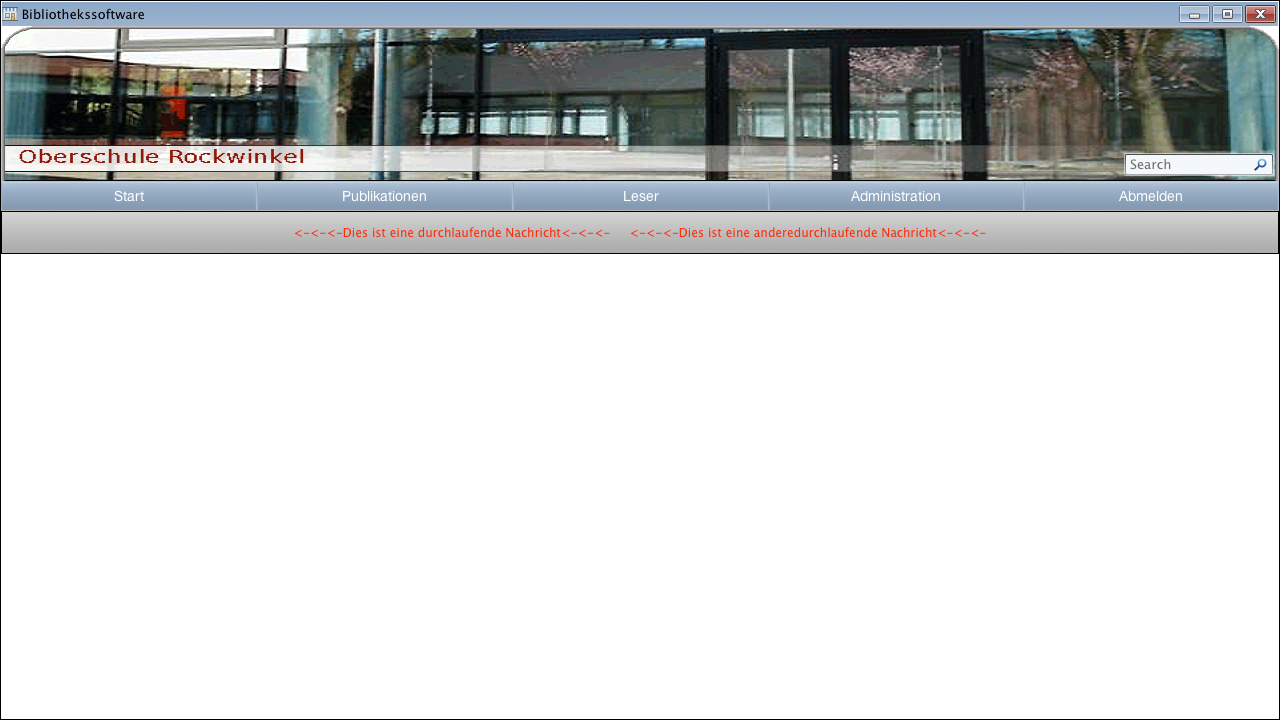
\includegraphics[width=1\textwidth]{WebApp-Screens/Startscreen-loggedIn.png}
  \label{startlog}
\end{figure}

\begin{table}[htbp]
\label{3}
\begin{tabular}{|l|p{10cm}|}
\hline 
\textbf{3} & \textbf{Startseite anzeigen} \\ \hline
\textbf{Akteure} & Bert Bib, Arnold Admin, Silke Schüler, Bart Besucher\\ \hline
\textbf{Ziel} & Der Akteur möchte die Startseite des Systems aufrufen  \\ \hline
\textbf{Vorbedingungen} & Das Programm wurde gestartet  \\ \hline
\textbf{Regulärer Ablauf} & 
1. Ein Benutzer drückt auf den Button Start \\
&2. Das System zeigt die Startseite an\\
\textbf{Varianten} & 
Anwendungsfall \ref{1} \\ \hline
\textbf{Nachbedingungen} & Es wird nun die Startseite angezeigt \\ \hline
\textbf{Fehler-/Ausnahmefälle} & keine
\end{tabular}
\end{table}

\begin{figure}[htbp]
\caption{Publikationsscreen von Silke Schüler oder Bart Besucher}
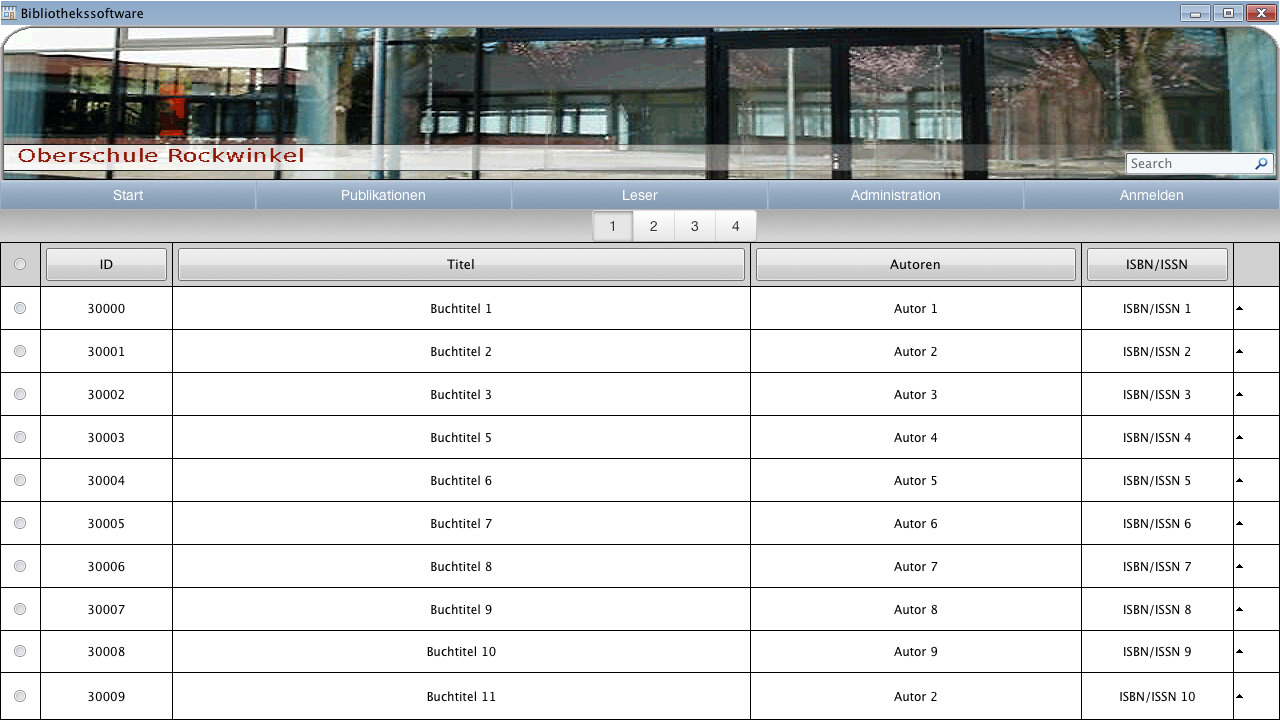
\includegraphics[width=1\textwidth]{WebApp-Screens/PublicationsscreenLogOut.png}
  \label{pub}
\end{figure}

\begin{table}[htbp]
\label{4}
\begin{tabular}{|l|p{10cm}|}
\hline 
\textbf{4} & \textbf{Publikationen anzeigen} \\ \hline
\textbf{Akteure} & Bert Bib, Arnold Admin, Silke Schüler, Bart Besucher\\ \hline
\textbf{Ziel} & Der Akteur möchte die Startseite des Systems aufrufen  \\ \hline
\textbf{Vorbedingungen} & Das Programm wurde gestartet  \\ \hline
\textbf{Regulärer Ablauf} & 
1. Ein Benutzer drückt auf den Button Start \\
&2. Das System zeigt die Startseite an\\
\textbf{Varianten} & 
Anwendungsfall \ref{1} \\ \hline
\textbf{Nachbedingungen} & Es wird nun die Startseite angezeigt \\ \hline
\textbf{Fehler-/Ausnahmefälle} & keine
\end{tabular}
\end{table}

\subsection{Aktionen}
  {\em Hier sollten die gleichen Aktionen wie in den Anwendungsfällen
  genannt und genauer beschrieben werden. Mit anderen Worten: Die
  Anwendungsfälle müssen vollständig durch Ausführung von Aktionen aus
  dieser Liste durchführbar sein. Im Prinzip muss es z.B.\ für jeden
  Button/Menüpunkt/Link eine Aktion geben. Dabei ist zu beachten:
  \begin{itemize}
    \item Die Namen sollten sinnvoll und eindeutig sein.

    \item Die Parameter der Aktionen sollen angegeben werden. Hier
    sollen sprechende Namen verwendet werden. Eventuell müssen die
    Parameter auch genauer erläutert werden.

    \item Es müssen maximale Ausführungszeiten für jede Operation
    angegeben werden.
    
  \item Die Gruppierung und Sortierung sollte sinnvoll sein
    (z.B. alphabetisch).
  \end{itemize}

  Wenn Ihr z.B.\ irgendwo in Eurer GUI ein Suchfeld habt, in das Ihr
  den Namen eines Kunden eintragen könnt, und einen Button, welcher die
  Suche startet, dann wird es vermutlich eine Aktion {\bf Kunde
    suchen(name)} geben. Dies ist eine Funktion, die Euer System
  bereitstellt und die durch Anklicken des Buttons ausgelöst wird. Der
  Anwendungsfall {\bf Kunde suchen} verwendet dann diese Aktion,
  enthält aber zusätzlich die Beschreibung der Interaktion mit dem
  System.
  
  Dieser Abschnitt ist im Standard im Prinzip vorgesehen, weil hierzu
  grundsätzlich eine Aussage gemacht werden muss. Die Aktionen sind
  letztlich die Produktfunktionen, während die Anwendungsfälle die
  Interaktion zwischen Akteuren und System beschreiben. }

  
\subsection{Entwurfseinschränkungen}
\nurlangversion

{\em Wurde bereits in \ref{sec:Einschraenkungen} behandelt und muss
  daher hier nicht wiederholt werden. Falls aber eine detailliertere
  Beschreibung notwendig wäre, wäre hier der geeignete Ort.}
  

\subsection{Softwaresystemattribute}
  {\em Hier werden die sogenannten „nichtfunktionalen Anforderungen“
  spezifiziert. Dazu gehören beispielsweise:
  \begin{itemize}
    \item Performanz
    \item Zuverlässigkeit (Korrektheit, Robustheit, Ausfallsicherheit)
    \item Verfügbarkeit
    \item Sicherheit
    \item Wartbarkeit
    \item Portabilität
  \end{itemize}
}

{\em Die spezifizierten Systemattribute müssen hinreichend konkret und
  überprüfbar formuliert werden.}



\subsection{Weitere Anforderungen}
\nurlangversion

{\em In diesem Abschnitt können weitere relevante Anforderungen
  beschrieben werden, die in keine der oben genannten Abschnitte
  passen.}

\section{Anhang}
\nurlangversion

{\em Hier können weitere detailliertere Ergebnisse aus der Ist-Analyse
  oder andere Informationen, die zur Erstellung der Spezifikation
  gedient haben (z.B. Papierprototypen), angefügt werden.}

\end{document}
